\documentclass[12pt]{article}

% This is the preamble, load any packages you're going to use here
\usepackage{physics} % provides lots of nice features and commands often used in physics, it also loads some other packages (like AMSmath)
\usepackage{siunitx} % typesets numbers with units very nicely
\usepackage{enumerate} % allows us to customize our lists
\usepackage[a4paper, margin=2.5cm]{geometry}
\usepackage[german]{babel}
\usepackage{hyperref}
\usepackage{url}
\usepackage{listings}
\usepackage{xcolor}
\usepackage{graphicx}
\usepackage{float}
\usepackage{subcaption}

\definecolor{codegreen}{rgb}{0,0.6,0}
\definecolor{codegray}{rgb}{0.5,0.5,0.5}
\definecolor{codepurple}{rgb}{0.58,0,0.82}
\definecolor{backcolour}{rgb}{1,1,1}

\lstdefinestyle{mystyle}{
    backgroundcolor=\color{backcolour},   
    commentstyle=\color{codegreen},
    keywordstyle=\color{magenta},
    numberstyle=\tiny\color{codegray},
    stringstyle=\color{codepurple},
    basicstyle=\ttfamily\footnotesize,
    breakatwhitespace=false,         
    breaklines=true,                 
    captionpos=b,                    
    keepspaces=true,                 
    numbers=left,                    
    numbersep=5pt,                  
    showspaces=false,                
    showstringspaces=false,
    showtabs=false,                  
    tabsize=2
}
\lstset{style=mystyle}

\lstdefinelanguage[2]{protobuf}{%
    sensitive=true,%
    morecomment=[l]{//},%
    morecomment=[s]{/*}{*/},%
    morestring=[b]{"},%
    % For the keywords of Protocol Buffers
    % see https://developers.google.com/protocol-buffers/docs/proto
    morekeywords={enum,oneof,map,syntax,public,import,option,package,message,%
        group,optional,required,repeated,default,reserved,extend,extensions,%
        to,max,service,rpc,returns,true,false},%
    % Basic types
    % see https://developers.google.com/protocol-buffers/docs/proto#scalar
    morekeywords=[2]{%
        double,float,int32,int64,uint32,uint64,sint32,sint64,%
        fixed32,fixed64,sfixed32,sfixed64,bool,string,bytes},%
    % Options
    % taken from 'google/protobuf/descriptor.proto'
    morekeywords=[3]{%
        % Generic Options
        deprecated, uninterpreted_option,%
        % File Options
        java_package,java_outer_classname,java_multiple_files,%
        java_generate_equals_and_hash,java_string_check_utf8,optimize_for,%
        go_package,cc_generic_services,java_generic_services,%
        py_generic_services,cc_enable_arenas,obj_class_prefix,%
        csharp_namespace,%
        % Message Options
        message_set_wire_format,no_standard_descriptor_accessor,map_entry,%
        % Field Options
        ctype, packed,jstype,lazy,weak,%
        % Enum Options
        allow_alias}%
}
\lstalias[]{protobuf2}[2]{protobuf}


\begin{document}

\title{%
Convolutional LSTM zur Bewegungsvorhersage von Verkehrsteilnehmern \\
  \large Anwendungen der Künstlichen Intelligenz \\
    Sommersemester 2021}
\author{Armin Straller}
\date{\today}

\maketitle

\begin{abstract}
    Um vorausschauendes Fahren für Autonome Fahrzeuge zu ermöglichen, ist es notwendig die Bewegungen anderer Verkehrsteilnehmer vorherzusagen. 
    Da das Verhalten von Fußgängern, Radfahreren und Autofahrern oft auf Interaktion basiert oder von Ortspezifischen Mustern abhängt, 
    bietet es sich an ein Netzwerk mit historischen Informationen über das Verhalten der Verkehrsteilnehmer aufzubauen.
	Diese Arbeit beschäftigt sich mit einem solchen Netzwerk zur Bewegungsvorhersage von Verkehrsteilnehmern.
    Als Datengrundlage wurde der im Frühjahr 2021 veröffentlichte Waymo Open Motion Datensatz verwendet. 
    Das entwickelte Netzwerk verwendete bildbasierte Eingangsdaten welche eine gerasterte Darstellung der unterschiedlichen Szenarien verwendet.
    Ein LSTM bietet dann die Möglichkeit Daten eines vergangen Zeitraums in Kontext zu bringen und ein eine bildliche Repräsentation eines zukünftigen Zustands auszugeben. 
    Das aus der Arbeit resultierende Netzwerk ermöglicht grundlegende vorhersagen der Bewegungsrichtung ist aber zum aktuellen Entwicklungsstand nicht für den Einsatz in einem Autonomen Fahrzeug geeignet.
\end{abstract}

\section{Problemstellung}
    Die Problemstellung für die entwickelte Künstliche Intelligenz ist aus der Waymo Motion Prediction Challenge abgeleitet.
    Hierbei soll auf Basis der Verkehrsdaten aus einer vergangenen Sekunde eine prädiktion für die folgenden acht Sekunden erfolgen.
    Der dafür bereitgestellte Datensatz ist das Waymo Open Motion Dataset~\cite{ettinger2021large}. 
    Dieses umfasst 574~Stunden und 1750~km an Verkehrsinformation und bietet somit genug Informationen für das Training eines Neuronalen Netzwerks.

    \subsection{Datengrundlage}
        Im Datensatz von Waymo sind verschidene Informationen über die aktuelle Verkehrssituation enthalten. Diese können im Detail dem scenario.proto aus dem Anhang entnommen werden.
        Teil des Scenarios ist auch eine Karte deren Details in der map.proto Datei definiert sind.~\cite{waymo2021github}

        Auf die für diese Arbeit wichtigen Inhalte der Szenarien wird Kapitel über die \hyperref[sec:preprocessing]{Vorverarbeitung der Daten} eingegangen.

\newpage

\section{Related Work und Entstehung der Projektidee}
    Es haben sich bereits andere Arbeiten mit der Vorhersage von Bewegungen im Straßenverkehr beschäftigt. 
    Aufgrund der aktualität des Waymo Datensatzes sind zu diesem allerdings noch keine Veröffentlichungen bekannt. 
    Ein Datensatz mit ähnlichem Inhalt wurde für die Prediktion von anderen Fahrzeugen in der Arbeit von Jeong, Yonghwan verwendet. 
    Hierbei kam ein LSTM-RNN Netzwerk zum Einsatz.~\cite{Yonghwan2020}
    
    Auch die Arbeit von Wu, Jingyuan beschäftigt sich mit der Bewegungsvorhersage. 
    In diesem Fall geht es um Fußgänger und eine Karten- beziehungsweise Modellbasierte Methodik zur Vorhersage. 
    Diese verwendet ein Raster welches die Aufenthaltswahrscheinlichkeit der Fußgänger darstellt.~\cite{Jingyuan2018}

    \subsection{Convolutional LSTM basierte Bewegungsvorhersage}
    Auf Basis der aufgeführten Arbeiten und der zur verfügbaren Daten ist die grundlegende Idee für diese Arbeit entstanden. 
    Die Verkehrsinformationen werden in ein Raster eingetragen und in Bildform als Eingangsdaten für das Convolutional-LSTM verwendet.
    Hierdurch können die Karten- und Positionsdaten der Verkehrsteilnehmer in Relation gebracht werden. 
    Die Historie der Bewegung wird dann durch die Eingangsbreite des LSTMs dargestellt. 
    Das Keras Beispiel \grqq Next-Frame Video Prediction with Convolutional LSTMs\grqq ~\cite{Keras2021} dient als Grundlage für die Umsetzung.
    Da das Raster nur mit begrenzter Auflösung arbeitet kann es theoretisch vorkommen, dass das Autonome Fahrzeug 
    im Szenario das Raster verlässt. Um dies zu umgehen wird ein Ansatz eine Transformation des Szenarios in die Ego-Perspektive des autonomen Fahrzeugs beinhalten. 
    Im Folgenden wird daher von einer statischen oder dynamischen Darstellung gesprochen, wobei die dynamische Darstellung die Transformation in die Ego-Perspektive beinhaltet. 
    Um eine Prediktion von bis zu 8~Sekunden zu ermöglichen, soll das Modell erneute Prediktionen auf basis der bereits predizierten Bilder erstellen. 
    Dies wird wiederholt bis der benötigte Zeithorizont abgedeckt ist.  

\section{Vorverarbeitung der Daten}
\label{sec:preprocessing}
    Um die Informationen aus dem Waymo Open Motion Dataset in die Darstellungsform des Rasters zu bringen 
    sind einige Schritte notwendig. Diese werden im Folgenden erläutert. 
    \subsection{Einlesen des Protobuf} 
        Zunächst muss das Szenario aus dem scenario.proto Format eingelesen werden. 
        Hierfür werden Auszüge aus dem Waymo Open Dataset Motion Tutorial~\cite{Tutorial2021} verwendet. 
        Dabei werden allerdings nur die Einträge geladen die für die Rasterisierung der Objekte notwendig sind. 
        Es werden immer alle Zeitschritte geladen und anschließend konvertiert. 
        Dies beinhaltetd die vergangenen, den aktuellen und die zukünftigen Elemente des Protobufs.

    \subsection{Konvertierung der Karte}
        Die Karteninformation ist Teil des scenario.proto und wird in Form des map.proto in jedem Szenario bereitgestellt.
        Ein Auszug aus der map.proto Definition der in Listing~\ref{lst:maplisting} dargestellt wird zeigt diese Liste und die Definition der Punkte. 
        Hierbei ist zu beachten, dass die Punkte in Metern zu einem beliebigen Ursprung gegeben sind. 
        Die \grqq polyline\grqq~definiert dann ein Feature des Straßennetzwerks (im Beispiel für \grqq LaneCenter\grqq~). Diese ist eine Liste von \grqq MapPoints\grqq~welche Segemente zwischen aufeinanderfolgenden Punkten definieren.
        Da die Auflösung der Punkt groß genug ist werden diese Einfach in das Raster übertragen. 
        Sobald ein \grqq MapPoint\grqq~innerhalb eines Rasterelements liegt wird dieses entsprechend des Linientypen eingefärbt.
        \vspace{0.5cm}
        \begin{lstlisting}[language=protobuf2, caption=Auszug aus map.proto, label={lst:maplisting}]
        message LaneCenter {
            // ...
            repeated MapPoint polyline = 2;
        }
        message MapPoint {
            optional double x = 1;
            optional double y = 2;
            optional double z = 3;
        }
        \end{lstlisting}
        Im Abbildung~\ref{fig:stat_map} wird die Karte aus dem Szenario 38 des Validierungsdatensatzes dargestellt. 
        Die statische Repräsentation das Scenarios erfordert eine einmalige Konvertierung der Karte. 
        Diese bleibt dann für den gesamten Zeitraum des Szenarios konstant.

        \begin{figure}[H]
            \centering
            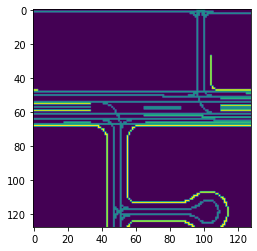
\includegraphics[width=0.3\textwidth]{example_static_map.png}
            \caption{Beispiel einer in das Raster übertragenen Karte}
            \label{fig:stat_map}
        \end{figure}

        \paragraph{Dynamische Darstellungsform der Karte}
            Für den Fall der dynamischen Darstellung der Karte muss diese bei jeder Bewegung des autonomen Fahrzeugs 
            in dessen Ego-Perspektive transformiert werden. Dadurch ergibt sich zum Beispiel bei einer Kurvenfahrt 
            eine Rotation und Translation der Karte. Dies wird in Abblidung~\ref{fig:dyn_maps} veranschaulicht. 
            Hier wird die Karte für die Zeitschritte -1~s also dem Start der Aufzeichnung, 0~s entsprechend dem gegenwärtigen Zeitschritt, 
            sowie den zukünftigen Zeitschritten +1~s und +2~s dargestellt. Datengrundlage ist das zweite Szenario des Validierungsdatensatzes. 
            
            \begin{figure}[H]
                \centering
                \begin{subfigure}[b]{0.18\textwidth}
                    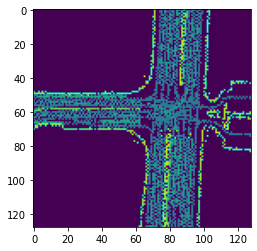
\includegraphics[width=\textwidth]{example_dynamic_map_0.png}
                    \caption{-1~s}
                \end{subfigure}
                ~
                \begin{subfigure}[b]{0.18\textwidth}
                    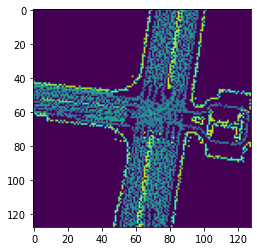
\includegraphics[width=\textwidth]{example_dynamic_map_10.png}
                    \caption{0~s}
                \end{subfigure}
                ~
                \begin{subfigure}[b]{0.18\textwidth}
                    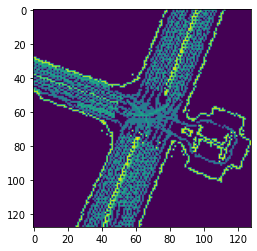
\includegraphics[width=\textwidth]{example_dynamic_map_20.png}
                    \caption{+1~s}
                \end{subfigure}
                ~
                \begin{subfigure}[b]{0.18\textwidth}
                    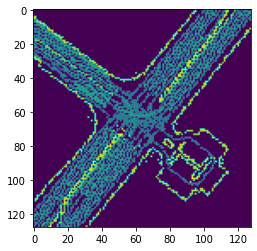
\includegraphics[width=\textwidth]{example_dynamic_map_30.png}
                    \caption{+2~s}
                \end{subfigure}
                ~
                \begin{subfigure}[b]{0.18\textwidth}
                    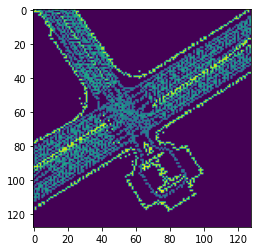
\includegraphics[width=\textwidth]{example_dynamic_map_40.png}
                    \caption{+3~s}
                \end{subfigure}
                \caption{Beispiel für eine dynamische gerasterte Karte}\label{fig:dyn_maps}
            \end{figure}

    \subsection{Konvertierung der Objekte}
        Der Protobuf enthält Informationen über die Größe sowie globale Position und Orienierung der Objekte. 
        Dadurch können die vier 2D-Eckkoordinaten der Objekte berechnet werden. Um diese in das 2D-Raster zu übertragen wird die Grundfläche der Box entlang der Diagonale in  
        zwei Dreiecke aufgeteilt und anschließend in das Raster übertragen. Wenn Objekte kleiner als ein Rasterelement sind, werden sie auf ein ganzes Rasterelement übertragen. 
        So kann sichergestellt werden, dass alle Objekte in der Darstellung repräsentiert werden.
        Die Definition der Objekte im Protobuf wird in Listing~\ref{lst:objectlisting} aufgeführt. 
        Das \grqq valid\grqq~Flag gibt an ob die Daten verwertbar sind. 
        Ist dieses für einen Zeitschritt nicht wahr, wird das Objekt für den zugehörigen Schritt nicht in das Raster übertragen.
        \vspace{0.5cm}
        \begin{lstlisting}[language=protobuf2, caption=Auszug aus scenario.proto, label={lst:objectlisting}]
        message ObjectState {
            optional double center_x = 2;
            optional double center_y = 3;
            optional double center_z = 4;
            
            optional float length = 5;
            optional float width = 6;
            optional float height = 7;

            optional float heading = 8;

            optional bool valid = 11;
        }
        \end{lstlisting}
        Im Abbildung~\ref{fig:stat_objects} werden Ausschnitte aus dem gesamten Szenario 38 des Validierungsdatensatzes dargestellt.
        Die Objekte werden entsprechend ihrer globalen Position dem Raster hinzugefügt.
        Da bei der Erstellung der Bilder für die Einfärbung eine Heatmap verwendet wir, werden stets die höchsten Werte in der hellsten Farbe dargestellt. 
        Deshalb ist die Karte in Abbildung~\ref{fig:stat_map} auch deutlich heller eingezeichnet als in Abbildung~\ref{fig:stat_objects}.

        \begin{figure}[H]
            \centering
            \begin{subfigure}[b]{0.18\textwidth}
                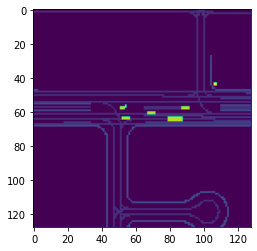
\includegraphics[width=\textwidth]{example_static_objects_0.png}
                \caption{-1~s}
            \end{subfigure}
            ~
            \begin{subfigure}[b]{0.18\textwidth}
                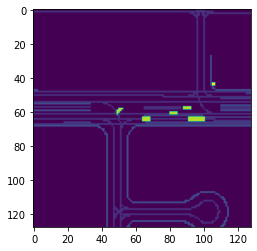
\includegraphics[width=\textwidth]{example_static_objects_10.png}
                \caption{0~s}
            \end{subfigure}
            ~
            \begin{subfigure}[b]{0.18\textwidth}
                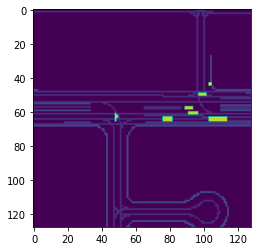
\includegraphics[width=\textwidth]{example_static_objects_20.png}
                \caption{+1~s}
            \end{subfigure}
            ~
            \begin{subfigure}[b]{0.18\textwidth}
                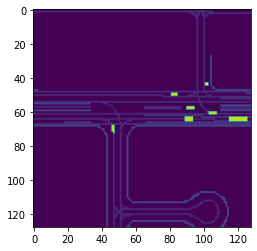
\includegraphics[width=\textwidth]{example_static_objects_30.png}
                \caption{+2~s}
            \end{subfigure}
            ~
            \begin{subfigure}[b]{0.18\textwidth}
                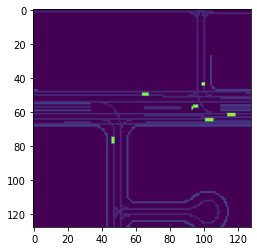
\includegraphics[width=\textwidth]{example_static_objects_40.png}
                \caption{+3~s}
            \end{subfigure}
            \caption{Beispiel für Objekte auf statischer Karte}\label{fig:stat_objects}
        \end{figure}

        \paragraph{Dynamische Darstellungsform für Objekte}
        Bei der dynamischen Darstellungsform, müssen alle Objekte auf Basis der aktuellen Position des autonomen Fahrzeugs 
        in dessen lokales Koordinatensystem transformiert werden. Die Information darüber welches Fahrzeug das autonom agierende ist, 
        kann ebenfalls dem Protobuf entnommen werden. Die dynamische Darstellung der Objekte wird in Abbildung~\ref{fig:dyn_objects} anhand des zweiten Scenarios aus dem Validierungsdatensatz gezeigt.
        
        \begin{figure}[H]
            \centering
            \begin{subfigure}[b]{0.18\textwidth}
                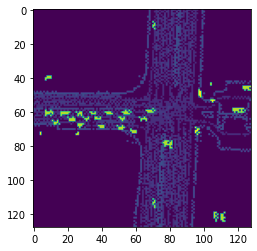
\includegraphics[width=\textwidth]{example_dynamic_objects_0.png}
                \caption{-1~s}
            \end{subfigure}
            ~
            \begin{subfigure}[b]{0.18\textwidth}
                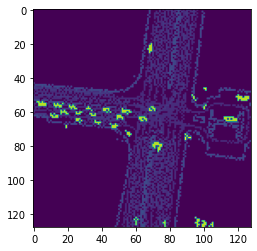
\includegraphics[width=\textwidth]{example_dynamic_objects_10.png}
                \caption{0~s}
            \end{subfigure}
            ~
            \begin{subfigure}[b]{0.18\textwidth}
                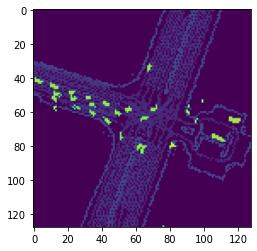
\includegraphics[width=\textwidth]{example_dynamic_objects_20.png}
                \caption{+1~s}
            \end{subfigure}
            ~
            \begin{subfigure}[b]{0.18\textwidth}
                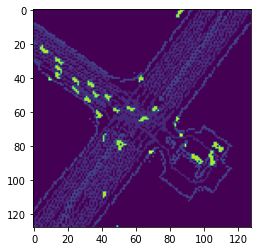
\includegraphics[width=\textwidth]{example_dynamic_objects_30.png}
                \caption{+2~s}
            \end{subfigure}
            ~
            \begin{subfigure}[b]{0.18\textwidth}
                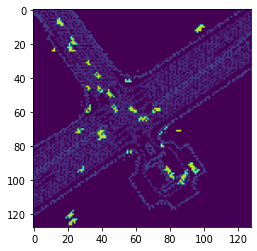
\includegraphics[width=\textwidth]{example_dynamic_objects_40.png}
                \caption{+3~s}
            \end{subfigure}
            \caption{Beispiel für Objekte in dynamischer Darstellungsform}\label{fig:dyn_objects}
        \end{figure}

    \subsection{Speicherung der Trainings- und Validierungsdaten}
        Die konvertierten Daten werden für das Training des ConvLSTM Netzwerks in einer Ordnerstruktur abgelegt. 
        Diese beinhaltet einen Ordner für jedes Szenario. 
        Ordner bei denen die statische Darstellungsform verwendet wurde tragen den prefix \grqq static\textunderscore\grqq .
    \subsection{Probleme bei der Datengenerierung} 
        \paragraph{Fehler durch Rasterisierung} Die Rasterisierung dazu führt, dass Objekte nur mit der Rasterauflösung von 0.5~m positioniert sein können. 
        Deshalb kann es vorkommen, dass Objekte von einem Zeitschritt zum nächsten um die Rasterauflösung springen. 
        Dies führt bei einer nur geringen Bewegung, die allerdings die grenze zum nächsten Feld des Rasters überschreitet, zu großen Fehlern. 
        \paragraph{Konvertierungszeit} Durch die große Datenmenge der Protobufs und die ineffiziente Programmierung des Konvertierungsalgorithmus, 
        benötigt dieser zwischen 150~s und 200~s für die Konvertierung eines Szenarios.

\section{ConvLSTM für Bewegungsvorhersage}
    Das Convolutional LSTM bietet die Möglichkeit die Informationen auf Bildebene miteinander zu assoziieren 
    und in einen Zeitlichen Kontext zu bringen. Aufgrund dieser Eigenschaften bietet es eine gute Grundlage für den Anwendungsfall.
    \subsection{Modell}
        Für die Erstellung des Modells wurden tensorflow und keras eingesetzt. 
        Diese beiden Bibliotheken bieten die Möglichkeit mit einfachen Interfaces komplexe funktionalitäten umzusetzen.
        \subsubsection{Architektur}
            Das Netzwerk folgt der Architektur die in Listing~\ref{lst:summarylisting} dargestellt ist. Es besteht aus mehreren Convolutional LSTM Layern die über eine jeweils kleinere Fenstergröße verfügen.
            Um die generalisierung des Netzwerks zu verbessern und geringere Trainingszeiten zu ereichen werden Normalisierungs Layers eingefügt. 
            Die Netzwerkarchitektur wurde Aufgrund der guten Ergebnisse, die im Beispiel von Keras~\cite{Keras2021} erziehlt wurden, gewählt.
            \begin{lstlisting}[caption=Ausgabe des model.summary() Aufrufs, label={lst:summarylisting}, basicstyle=\tiny, numbers=none]
                    _________________________________________________________________
                    Layer (type)                 Output Shape              Param #   
                    =================================================================
                    conv_lst_m2d (ConvLSTM2D)    (None, 10, 128, 128, 128) 1651712   
                    _________________________________________________________________
                    batch_normalization (BatchNo (None, 10, 128, 128, 128) 512       
                    _________________________________________________________________
                    conv_lst_m2d_1 (ConvLSTM2D)  (None, 10, 128, 128, 128) 1180160   
                    _________________________________________________________________
                    batch_normalization_1 (Batch (None, 10, 128, 128, 128) 512       
                    _________________________________________________________________
                    conv_lst_m2d_2 (ConvLSTM2D)  (None, 10, 128, 128, 128) 131584    
                    _________________________________________________________________
                    batch_normalization_2 (Batch (None, 10, 128, 128, 128) 512       
                    _________________________________________________________________
                    conv3d (Conv3D)              (None, 10, 128, 128, 1)   3457      
                    =================================================================
                    Total params: 2,968,449
                    Trainable params: 2,967,681
                    Non-trainable params: 768
                    _________________________________________________________________
            \end{lstlisting}

            Insgesamt beinhaltet das Modell 2967681 trainierbare Parameter. 
            Auf dem System welches zum Training verwendet werden soll werden diese Parameter durch float32 repräsentiert welcher 4~Byte im Speicher benötigt.
            Dies führt auf Basis der Berechnung in Formel~\ref{memory-size} zu einem Speicherbedarf von 11.87~GB. 
            \begin{align}
                2967681 \cdot 4~Bytes = 11.87~GB
                \label{memory-size}
            \end{align}
    \subsection{Training}
        Beim Training wurde zunächst die dynamische Darstellungsform der Szenarioen Verwendet. 
        Diese lieferte allerdings transformierte und rotierte Bilder bei denen für eine erneute Prediktion die Transformation und Rotation bestimmt werden musste. 
        Um diesen Prozess zu vereinfachen wurde deshalb das Training auf die statische Darstellungsform umgestellt.
        \subsubsection{Spezifische Loss-Funktion}
	        Da die Trainingsbilddaten viele Bereiche enthalten die für die Performance des Netzwerks nicht relevant sind, 
            wurde eine für das Netzwerk zugeschnittene Loss funktion Implementiert. 
            Diese Analysiert den Mean-Squared Error in verschiedenen Bereichen des predizierten Bildes. 
            \paragraph{Zukünftige Aufenthaltsorte von Objekten} Hier wird der Mean-Squared Error für die Pixel in denen Sich das Objekt aufhalten sollte berechnet. 
            Dieser wird mit einem Verhältnis von 80~\% gewichtet.
            \paragraph{Hintergrund und Karte} Über den Rest des Bildes wird ebenfalls ein Mean-Squared Error Wert berechnet. 
            Dies ist notwendig, da das Netzwerk sonst das gesamte Bild in Objektfarbe einfärben würde und dadurch eine hohe Genauigkeit erreicht.
            Der Wert wird dann mit 20~\% gewichtet.
        \subsubsection{Generierung der Trainingsdaten zur Laufzeit}
            Um das Training mit der gesamten Menge der Szenariodaten auf einer Platform mit beschränkten Ressourcen zu ermöglichen wurde ein Gernerator für Trainingsdaten implementiert.
            Dieser verwendet eine Datenstruktur die Dateipfade enthält und lädt die Trainingsdaten immer erst zur Lauftzeit in den Arbeitsspeicher.
        \subsubsection{Gradient Accumulation}
            Zudem wurde das Prinzip der Gradient Accumulation eingesetzt um den auf der Grafikkarte benötigten Speicherplatz zu reduzieren. 
            Hierbei werden die Batches die zum Training verwendet werden aufgeteilt. Diese werden dann nacheinander trainiert. Der resultierende Gradient wird dann im Anschluss akkumuliert.
            Dadurch entsteht beim Training der gleiche Effekt wie bei größeren Batch Größen. Der Speicherbedarf bleibt jedoch konstant klein.~\cite{Ttowardsdatascience2021}

\section{Ergebnisse}
    Der Ansatz ein Convolutional LSTM für die Bewegungsvorhersage einzusetzen zeigt erste vielversprechende Ergebnisse.
    Alle Prediktionen von Abbildung~\ref{fig:out_low_dens} bis Abbildung~\ref{fig:out_static_brake} dienen der Veranschaulichung der Performance des ConvLSTMs. 
    Besser Sichtbar sind diese jedoch in Form von Animationen. Diese können in dem beigefügten Jupyter Notebook inference.ipynb erzeugt werden. 
    Hierbei wird die Datenkonvertierung nicht mehr durchgeführt. 

    Für die Erstellung der Prediktionen wurde das Trainierte Convolutional LSTM verwendet. Für Prediktionen die über 100~ms hinaus gehen, wurde das Ergebnis als jeweils 10tes Bild wieder in das Netzwerk eingespeist.
    
    
    \pagebreak
    \subsection{Scenario mit geringer Dichte an Objekten}
        In Szenarien mit gerninger Fahrzeugdichte passen die Ausgaben des Modells grundlegend zu den Refernzdaten des Validierungsdatensatzes.
        Dies ist im folgenden Beispiel erkennbar. Besonders in Abblidung~\ref{fig:out_low_dens} bei +1~s ist gut zu sehen wie die Bewegung der drei größeren Objekte weiter prediziert wird. 

        \begin{figure}[H]
            \centering
            \begin{subfigure}[b]{0.18\textwidth}
                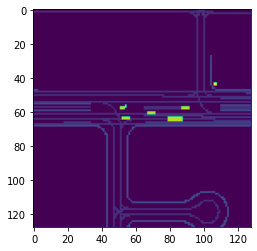
\includegraphics[width=\textwidth]{output_low_dens_0.png}
                \caption{-1~s}
            \end{subfigure}
            ~
            \begin{subfigure}[b]{0.18\textwidth}
                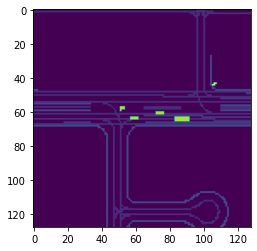
\includegraphics[width=\textwidth]{output_low_dens_1.png}
                \caption{-0.5~s}
            \end{subfigure}
            ~
            \begin{subfigure}[b]{0.18\textwidth}
                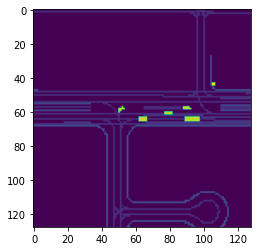
\includegraphics[width=\textwidth]{output_low_dens_2.png}
                \caption{0~s}
            \end{subfigure}
            ~
            \begin{subfigure}[b]{0.18\textwidth}
                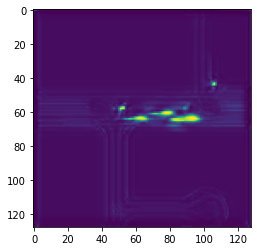
\includegraphics[width=\textwidth]{output_low_dens_3.png}
                \caption{+0.1~s}
            \end{subfigure}
            ~
            \begin{subfigure}[b]{0.18\textwidth}
                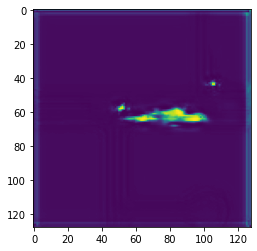
\includegraphics[width=\textwidth]{output_low_dens_4.png}
                \caption{+1~s}
            \end{subfigure}
            \vspace{1cm}
            \begin{subfigure}[b]{0.6\textwidth}
                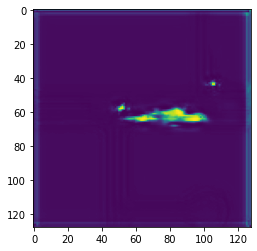
\includegraphics[width=\textwidth]{output_low_dens_4.png}
                \caption{Vergrößerte Darstellung der Prediktion bei +1~s}
            \end{subfigure}
            \caption{Beispiel für Szenario mit geringer Objektdichte}\label{fig:out_low_dens}
        \end{figure}

    \pagebreak
    \subsection{Komplexes Szenario mit unterschiedlichen Bewegungsrichtungen} 
        Für den Fall eines komplexeren Szenarios mit vielen Objekten, unterschiedlichen Fahrtrichtungen und komplexeren Kartensituationen, liefert das Modell unzuverlässige Ergebnisse.
        In der Abbildung~\ref{fig:out_opposite} werden alle Objekte in die gleiche Richtung prediziert. Dies ist für die in der Abbildung oben liegende Fahrspur falsch.

        \begin{figure}[H]
            \centering
            \begin{subfigure}[b]{0.18\textwidth}
                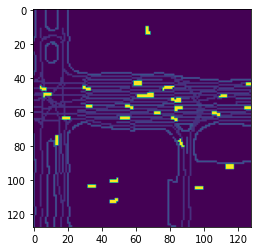
\includegraphics[width=\textwidth]{output_opposite_0.png}
                \caption{-1~s}
            \end{subfigure}
            ~
            \begin{subfigure}[b]{0.18\textwidth}
                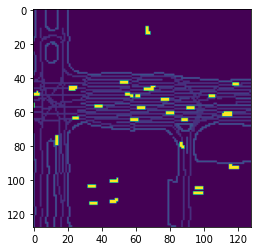
\includegraphics[width=\textwidth]{output_opposite_1.png}
                \caption{-0.5~s}
            \end{subfigure}
            ~
            \begin{subfigure}[b]{0.18\textwidth}
                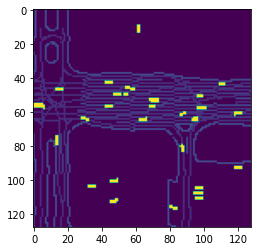
\includegraphics[width=\textwidth]{output_opposite_2.png}
                \caption{0~s}
            \end{subfigure}
            ~
            \begin{subfigure}[b]{0.18\textwidth}
                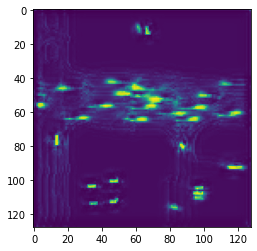
\includegraphics[width=\textwidth]{output_opposite_3.png}
                \caption{+0.1~s}
            \end{subfigure}
            ~
            \begin{subfigure}[b]{0.18\textwidth}
                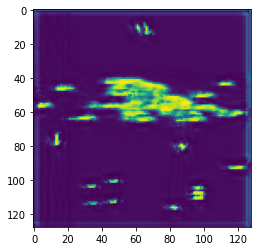
\includegraphics[width=\textwidth]{output_opposite_4.png}
                \caption{+1~s}
            \end{subfigure}
            \vspace{1cm}
            \begin{subfigure}[b]{0.6\textwidth}
                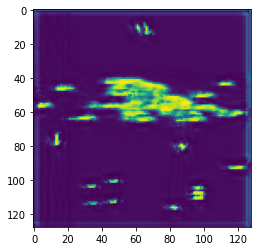
\includegraphics[width=\textwidth]{output_opposite_4.png}
                \caption{Vergrößerte Darstellung der Prediktion bei +1~s}
            \end{subfigure}
            \caption{Beispiel für komplexes Szenario mit Gegenverkehr}\label{fig:out_opposite}
        \end{figure}

    \pagebreak
    \subsection{Szenario mit statischem Hindernis am Straßenrand} 
        Ein Beispiel bei dem bessere Ergebnisse erziehlt wurden ist das folgende Szenario bei dem die Fahrzeuge für eine statisches Hindernis am Straßenrand verzögern müssen. 
        Hier liegen die Prediktionen relativ nah an den Referenzdaten. In Abbildung~\ref{fig:out_static_brake} wird zudem ersichtlich, dass die predizierte Positionsänderung der Objekte nicht für das gesamte Ausgangsbild gleich ist. 
        Objekte die zu Beginn des Szenarios schneller sind bewegen sich noch weiter als Objekte die bereits langsam sind und innerhalb des predizierten Zeitraumes zum Stillstand kommen. 

        \begin{figure}[H]
            \centering
            \begin{subfigure}[b]{0.18\textwidth}
                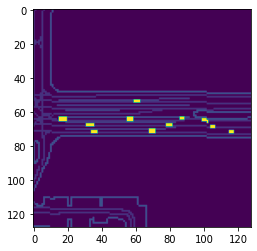
\includegraphics[width=\textwidth]{output_static_brake_0.png}
                \caption{-1~s}
            \end{subfigure}
            ~
            \begin{subfigure}[b]{0.18\textwidth}
                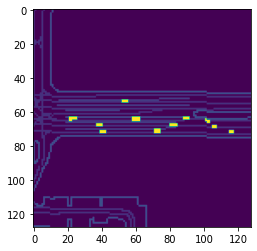
\includegraphics[width=\textwidth]{output_static_brake_1.png}
                \caption{-0.5~s}
            \end{subfigure}
            ~
            \begin{subfigure}[b]{0.18\textwidth}
                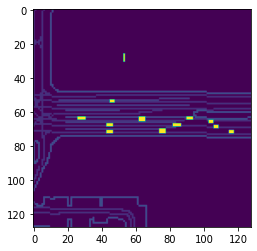
\includegraphics[width=\textwidth]{output_static_brake_2.png}
                \caption{0~s}
            \end{subfigure}
            ~
            \begin{subfigure}[b]{0.18\textwidth}
                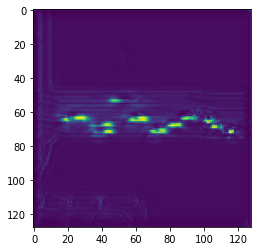
\includegraphics[width=\textwidth]{output_static_brake_3.png}
                \caption{+0.1~s}
            \end{subfigure}
            ~
            \begin{subfigure}[b]{0.18\textwidth}
                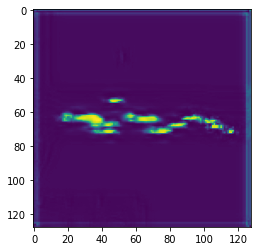
\includegraphics[width=\textwidth]{output_static_brake_4.png}
                \caption{+1~s}
            \end{subfigure}
            \vspace{1cm}
            \begin{subfigure}[b]{0.6\textwidth}
                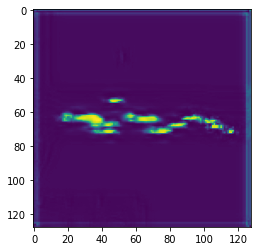
\includegraphics[width=\textwidth]{output_static_brake_4.png}
                \caption{Vergrößerte Darstellung der Prediktion bei +1~s}
            \end{subfigure}
            \caption{Beispiel für Szenario mit Geschwindigkeitsdifferenz}\label{fig:out_static_brake}
        \end{figure}
    \pagebreak
    \subsection{Beobachtete Probleme bei der Prediktion}
        Folgende Probleme wurden bei der Prediktion in kombination mit der Datenaufbereitung fetstgestellt.
        
        \paragraph{Probleme durch nichtlineare Einfärbung bei Rasterisierung} Da bei der Datenverarbeitung eine 
        nichtlineare Funktion zum einfärben der Objekte und Kartendaten verwendet wurde, unterscheiden sich die Trainingsdaten 
        zum Teil stark in der Intesität. Dies fürhrt dazu, dass das Decoding der Bildinformationen in Positionsdaten auf 
        Basis von klassischer Bildverarbeitung nur aufwändig möglich ist. Daher kann im Rahmen dieses Projketes keine aussagekräftige 
        Auswertung über die Genauigkeit der Prediktionen erfolgen.

        Durch inkonsequente Einfärbung der Trainingsdaten ist es zudem nicht möglich die Daten aufzubereiten und mehrfache Prediktionen durchzuführen.
        Hierdurch sollte ursprünglich eine gesamte Vorausschau von 8~Sekunden erreicht werden.

        \paragraph{Verbesserungsmöglichkeiten bei der spezifischen Loss-Funktion} Die Kartendaten hinterlassen Fragmente bei der Vorhersage. 
        Diese können vermutlich durch die Bearbeitung der Loss-Funktion beeinflusst und reduziert werden.
        \paragraph{Training mit längeren Zeitabschnitten} Aufgrund der limiterten Hardwareleistung wurden nur beim Training mit dem ersten 
        Zeitschritte der 1000~Scenarios verwertbare Ergebnisse erziehlt. Bei einem Training mit allen Zeitschritten der 1000~Szenarios ist zu erwarten, 
        dass bessere Ergebnisse erziehlt werden können.

    \subsection{Lessons Learned und Future Work}
        \begin{itemize}
            \item Gradient Accumulation ermöglicht den Speicherbedarf für Zwischenergebnisse auf der GPU zu verringern.
            \item Der Rechenaufwand für die Rasterisierung der Daten, sowie der benötigte Speicherbedarf für Convolutional LSTMs sollte nicht unterschätzt werden.
            \item Die Inference Zeit ist deutlich schlechter als bei einer Bild-Klassifikation. Dies liegt an der größe des Netzwerks und der Menge der Eingangsdaten. Dies sollte für die praktische Verwendbarkeit des ConvLSTM+Raster Ansatzes berücksichtigt werden. 
            \item Durch höhere Auflösung des Rasters könnten Objekte besser unterschieden und unabhängig voneinander prediziert werden. Dies führt allerdings zu einer geringeren betrachtbaren Kartengröße oder zu einem größeren und langsameren Netzwerk.
        \end{itemize}
\pagebreak
\bibliography{motion-prediction}{}
\bibliographystyle{ieeetr}

\end{document}